\documentclass[cs4size,a4paper]{ctexart}   
\usepackage{amlnote}

%===正文开始===
\begin{document}
\fancyhead[C]{\zihao{5} \kaishu 计算方法课程综合项目报告}
%===首页===
\begin{titlepage}
	\begin{center}
		% Upper part of the page
		
\includegraphics[width=0.33\textwidth]{logo}\\[1cm]
		\textsf{\LARGE\bfseries Beijing University of Chemical Technology}\\[1.0cm]
		\textsf{\Large\bfseries Course Project Report}\\[0.5cm]
		% Title
		\HRule \\[0.8cm]
		{\huge \bfseries 计算方法课程综合项目报告}\\[0.4cm]
		\HRule \\[0.7cm]
		% Author
		\textsc{Chen Yong}
		\tableofcontents
		\vfill
		% Bottom of the page
		{创建日期:2023年10月15日}\\
		{更新日期:\today}
	\end{center}
\end{titlepage}

%===第一章===
\newpage
\section{项目描述}
\subsection{散布熵(Dispersion Entropy, DispEn)}
散布熵(Dispersion Entropy)是一种用于衡量信号离散程度或波动性的指标。它通常用于信号处理、数据分析和生物医学领域。
散布熵的意义包括以下几个方面:
\begin{enumerate}[\quad\quad(1)]
	\item 衡量信号的波动性:
	      散布熵可以提供关于信号的波动程度的信息。对于具有不同波动性的信号,其散布熵值也会有所区别。
	\item 用于信号特征提取:
	      散布熵可以作为信号的特征,用于区分不同类型的信号。比如,在生物医学领域中,可以使用散布熵来分析心电图、脑电图等生理信号的波动性特征。
	\item 检测异常或异常事件:
	      在某些情况下,散布熵可以用于检测信号中的异常或突发事件,因为异常事件通常会导致信号的波动性增加。
	\item 用于状态监测和诊断:
	      在工程和医学应用中,散布熵可以用于监测设备状态或者对某些疾病进行诊断。例如,对机械设备振动信号的散布熵分析可以用于预测设备的健康状况。
	\item 信号预处理和特征选择:
	      在信号处理中,可以使用散布熵来进行信号预处理或者作为特征进行后续的分析和处理。
	\item 与其他熵相关指标结合使用:
	      散布熵可以与其他熵相关的指标(如信息熵、样本熵等)一起使用,以提供更全面的信号特征描述。
\end{enumerate}
\subsection {测试数据}
signal01.txt
\subsection {源代码库}
\url https://github.com/MattWillFlood/EntropyHub
\subsection{运行代码}
\emph{Matlab代码}
\begin{lstlisting}
% Read data from file
filename = 'C:\Users\123\Desktop\计算方法\2\其他数据集\signal01.txt';
Sig = load(filename);

% Call the MATLAB function
[Dispx_matlab, RDE_matlab] = DispEn(Sig);

% Display the results
disp('MATLAB Results:');
disp(['Dispersion Entropy (Dispx): ', num2str(Dispx_matlab)]);
disp(['Reverse Dispersion Entropy (RDE): ', num2str(RDE_matlab)]);
\end{lstlisting}

\emph{Cpp代码}
\begin{lstlisting}
#include <bits/stdc++.h>
using namespace std;

double normalCDF(double value); // 计算NCDF
double Dispn(vector<double> &x, int c, int m, int d);

int main()
{
	// 从文件中读取向量
	vector<double> x;
	ifstream inputFile("signal01.txt");
	if (!inputFile.is_open())
	{
		cerr << "Error opening file.\n";
		return 1;
	}
	double value;
	while (inputFile >> value)
		x.push_back(value);
	inputFile.close();

	int c, m, d;
	cout << "Please enter ..." << endl;
	cout << "c = ";
	cin >> c;
	cout << "m = ";
	cin >> m;
	cout << "d = ";
	cin >> d;

	cout << "C++ Results:" << endl;
	cout << "Dispersion Entropy (Dispx): " << Dispn(x, c, m, d) << endl;
	cout << "Reverse Dispersion Entropy (RDE): " << Dispn(x, c, m, d) / pow(c, m) << endl;
	return 0;
}
\end{lstlisting}

\newpage
\section{项目报告}
\subsection{算法描述}
% 这里放入列表内容
DE是为了解决相同振幅的问题而提出的。DE是一种基于符号的熵方法,对于长度为$L$的一维的时间序列数据$X=\{x_1,x_2,\cdots,x_L\}$,DE熵计算如下:
\begin{enumerate}[\quad\quad(1)]
	\item 首先,对给定的输入序列$X$,由其正态累积分布函数(NCDF)生成新的时间序列$Y =\{y_1, y_2,\cdots,y_L\}$,并且$y_j\in[0, 1]$。
	      \begin{align}
		      y_j=\frac{1}{\sigma\sqrt{2\pi}}\int_{-\infty}^{x_i}e^{\frac{-(t-\mu)^2}{2\sigma^2}}dt
	      \end{align}
	      然后,采用线性算法将$y_j (j = 1, 2,\cdots , L)$映射到$c$个类,其中$1$到$c$是整数索引。信号中每个映射的元素表示为:
	      \begin{align}
		      z_j^c=Round(c\cdot y_j+0.5)
	      \end{align}
	      其中$z_j^c$是分类时间序列的第$j$个元素,$Round(\cdot)$标识$Round$舍入操作。
	\item 对于嵌入维数$m$,类数目$c$和时间延迟$d$,嵌入向量$z_i^{m,c}$按下式构造:
	      \begin{align}
		      z_i^{m,c}=\{z_i^c,z_{i+d}^c,\cdots,z_{i+(m-1)d}^c\}
	      \end{align}
	      其中$i=1,2,\cdots,L-(m-1)d$。然后,每个$z_i^{m,c}$映射为一个分散模式(DispersionPattern)$\pi_{\nu_0,\nu_1,\cdots,\nu_{m-1}}$,$z_i^c=\nu_0,z_{i+d}^c=\nu_1,\cdots,z_{i+(m-1)d}^c=\nu_{m-1}$。每一$z_i^{m,c}$可行分散模式总数为$c^m$。
	\item 每个分散模式的相对频率可按下式计算:
	      \begin{align}
		      p(\pi_{\nu_0,\nu_1,\cdots,\nu_{m-1}})=\frac{Number \ \{i|i\leq-(m-1)d,z_i^{m,c} \ has \ type \ \pi_{\nu_0,\nu_1,\cdots,\nu_{m-1}}\}}{L-(m-1)d}
	      \end{align}
	      注意$L-(m-1)d$是嵌入向量的总数。
	\item 最后,DE的类数为$c$,嵌入维数$m$和时间延迟$d$,根据Shannon熵定义,可计算分散熵为:
	      \begin{align}
		      DE(X,m,c,d)=-\sum_{\pi=1}^{c_m}p(\pi_{\nu_0,\nu_1,\cdots,\nu_{m-1}})\ln (p(\pi_{\nu_0,\nu_1,\cdots,\nu_{m-1}}))
	      \end{align}
\end{enumerate}

\subsection{算法代码}
\emph{Matlab原型代码}
% 这里放原型代码





\begin{lstlisting}
function [Dispx, RDE] = DispEn(Sig, varargin)
narginchk(1,15)
Sig = squeeze(Sig);

p = inputParser;
Chk = @(x) isnumeric(x) && isscalar(x) && (x > 0) && (mod(x,1)==0);
Chk2 = @(x) isnumeric(x) && isscalar(x) && (x >= 0);
Chk3 = {'linear','kmeans','ncdf','finesort','equal'};
addRequired(p,'Sig',@(x) isnumeric(x) && isvector(x) && (length(x) > 8));
addParameter(p,'m',2,Chk);
addParameter(p,'tau',1,Chk);
addParameter(p,'c',3,@(x) isnumeric(x) && (x > 1) && (mod(x,1)==0));
addParameter(p,'Logx',exp(1),Chk2);
addParameter(p,'Fluct',false,@(x) islogical(x));
addParameter(p,'Norm',false,@(x) islogical(x));
addParameter(p,'Typex','ncdf',@(x) ischar(x) && any(validatestring(lower(x),Chk3)));
addParameter(p,'rho',1,Chk2);
parse(p,Sig,varargin{:})
m = p.Results.m; tau = p.Results.tau; c = p.Results.c;
Typex = p.Results.Typex; Logx = p.Results.Logx; Norm = p.Results.Norm;
rho = p.Results.rho;

N = length(Sig);
switch lower(Typex)
	case 'linear'
		Zi = discretize(Sig,linspace(min(Sig),max(Sig),c+1));
		
	case 'kmeans'    
		if size(Sig,2)>size(Sig,1)
			Sig = Sig';
		end        
		
		[Zx,Clux] = kmeans(Sig, c, 'MaxIter', 200);
		[~,xx] = sort(Clux);        Zi = zeros(1,N);
		for k = 1:c
			Zi(Zx==xx(k)) = k;
		end
		clear Clux Zx xx
		
	case 'ncdf'       
		Zx = normcdf(Sig,mean(Sig),std(Sig,1));
		Zi = discretize(Zx,linspace(0,1,c+1));     
		
	case 'finesort'
		Zx = normcdf(Sig,mean(Sig),std(Sig,1));
		Zi = discretize(Zx,linspace(0,1,c+1));
		Ym = zeros(N-(m-1)*tau, m);
		for n = 1:m
			Ym(:,n) = Zx(1+(n-1)*tau:N-((m-n)*tau));
		end
		Yi = floor(max(abs(diff(Ym,[],2)),[],2)/(rho*std(abs(diff(Sig)),1)));
		clear Zx Ym
		
	case 'equal'
		[~,ix] = sort(Sig);
		xx = round(linspace(0,N,c+1));
		Zi = zeros(1,N);
		for k = 1:c
			Zi(ix(xx(k)+1:xx(k+1))) = k;
		end
		clear ix xx
end

Zm = zeros(N-(m-1)*tau, m);
for n = 1:m
	Zm(:,n) = Zi(1+(n-1)*tau:N-((m-n)*tau));
end

if strcmpi(Typex,'finesort')
	Zm = [Zm Yi];
end
if p.Results.Fluct
	Zm = diff(Zm,[],2);
	if m < 2
		warning(['Fluctuation-based Dispersion Entropy'...
			' is undefined for m = 1. '...
			'An embedding dimension (m) > 1 should be used.'])       
	end
end

T = unique(Zm,'rows');
Nx = size(T,1);
Counter = zeros(1,Nx);
for n = 1:Nx
	Counter(n) = sum(~any(Zm - T(n,:),2));
end
Ppi = Counter(Counter~= 0)/length(Zm);
% RDE = sum(Ppi.^2) - (1/Nx);

if p.Results.Fluct
	RDE = sum((Ppi - (1/((2*c - 1)^(m-1)))).^2);
else
	RDE = sum((Ppi - (1/(c^m))).^2);
end

if round(sum(Ppi),4) ~= 1
	warning('Potential Error calculating probabilities')
end

Dispx = -sum(Ppi.*log(Ppi)/log(Logx));
if Norm
	%Dispx = Dispx/(log(Nx)/log(Logx));
	if p.Results.Fluct
		Dispx = Dispx/(log((2*c - 1)^(m-1))/log(Logx));
		RDE = RDE/(1 - (1/((2*c - 1)^(m-1))));
	else
		Dispx = Dispx/(log(c^m)/log(Logx));
		RDE = RDE/(1 - (1/(c^m)));
	end
end
end
	
\end{lstlisting}


\emph{Cpp实现代码}
% 这里放Cpp代码
\begin{lstlisting}
// 步骤(1)计算NCDF
double normalCDF(double value)
{
	return 0.5 * erfc(-value * M_SQRT1_2);
}
double Dispn(vector<double> &x, int c, int m, int d)
{
	// 步骤(1)映射到c个类
	vector<double> z;
	for (int i = 0; i < x.size(); i++)
		z.push_back(round(normalCDF(x[i]) * c + 0.5));

	// 步骤(2)映射为一个分散模式
	vector<vector<double>> zmc;
	for (int i = 0; i < x.size() - (m - 1) * d; i++)
	{
		vector<double> t;
		for (int j = i; j <= i + (m - 1) * d; j += d)
			t.push_back(z[j]);
		zmc.push_back(t);
	}

	// 步骤(3)求出相对频率
	map<vector<double>, double> mp;
	for (int i = 0; i < x.size() - (m - 1) * d; i++)
		mp[zmc[i]] += 1;

	vector<double> p;
	for (auto it = mp.begin(); it != mp.end(); it++)
		p.push_back(it->second / (x.size() - (m - 1) * d));

	// 步骤(4)得出结果
	double DE = 0;
	for (int i = 0; i < p.size(); i++)
		DE -= p[i] * log(p[i]);

	return DE;
}
\end{lstlisting}

\subsection{测试结果}
\subsubsection{原型测试结果}
% 这里放入图片文件
\begin{figure}[H]
	\small
	\centering
	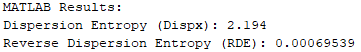
\includegraphics[width=0.8\textwidth]{matlabres}
	\caption{原型代码运行截图}
\end{figure}

\subsubsection{cpp测试结果}
% 这里放入图片文件
\begin{figure}[H]
	\small
	\centering
	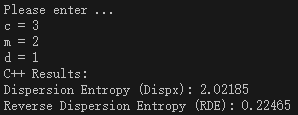
\includegraphics[width=0.8\textwidth]{cppresult}
	\caption{cpp代码运行截图}
\end{figure}


~\\
~\\
\subsection{问题及解决方案}
matlab和c++运行结果不一致有几个原因导致:(1)求NCDF的函数有误差(2)c, m, d的取值与原来的不同
~\\
~\\

\subsection{总结}
用Cpp代码实现散布熵
~\\
~\\


%===参考文献===
%\addcontentsline{toc}{section}{参考文献}
%\bibliographystyle{abbrv}     %论文引用格式
%\bibliography{E:/studio/wrtex/wrtkit/referbib/wholebiblio}


\begin{thebibliography}{99}
	\bibitem{A20}
	{\em \color{red}散布熵的意义} \url{https://blog.csdn.net/weixin_44943389/article/details/134126706}
	\bibitem{A20}
	{\em \color{red}散布熵(DE)的具体计算步骤} \url{https://zhuanlan.zhihu.com/p/539611038}
\end{thebibliography}
\end{document}
%===结束===
